\documentclass{G7-32}
\usepackage{xurl}
\sloppy

% Поля по нормоконтролю (верх/низ 20 мм, слева 30 мм, справа 15 мм); класс G7-32 уже подключает geometry — уточняем параметры
\geometry{a4paper,top=20mm,bottom=20mm,left=30mm,right=15mm}

% Абзацный отступ 1,25 см, без дополнительного интервала между абзацами одного стиля (методичка п. 2.2.10)
\setlength{\parindent}{1.25cm}
\setlength{\parskip}{0pt}

% Запрет висячих строк (нормоконтроль п. 35)
\widowpenalty=10000
\clubpenalty=10000

% Настройки стиля ГОСТ 7-32
% Для начала определяем, хотим мы или нет, чтобы рисунки и таблицы нумеровались в пределах раздела, или нам нужна сквозная нумерация.
% \EqInChapter % формулы будут нумероваться в пределах раздела
% \TableInChapter % таблицы будут нумероваться в пределах раздела
% \PicInChapter % рисунки будут нумероваться в пределах раздела

% Добавляем гипертекстовое оглавление в PDF
\usepackage[
bookmarks=true, colorlinks=true, unicode=true,
urlcolor=black,linkcolor=black, anchorcolor=black,
citecolor=black, menucolor=black, filecolor=black,
]{hyperref}

\urlstyle{same}

\usepackage{pdfpages}
\usepackage{pdflscape}

% Изменение начертания шрифта --- после чего выглядит таймсоподобно.
% apt-get install scalable-cyrfonts-tex

% \IfFileExists{cyrtimes.sty}
%     {
        % \usepackage{cyrtimespatched}
%     }
%     {
%         % А если Times нету, то будет CM...
%     }

\usepackage{graphicx}   % Пакет для включения рисунков
\usepackage{grffile}    % поддержка имён файлов с пробелами
\graphicspath{{images/}}

% С такими оно полями оно работает по-умолчанию:
% \RequirePackage[left=20mm,right=10mm,top=20mm,bottom=20mm,headsep=0pt]{geometry}
% Если вас тошнит от поля в 10мм --- увеличивайте до 20-ти, ну и про переплёт не забывайте:

% Пакет Tikz
\usepackage{tikz}
\usetikzlibrary{arrows,positioning,shadows}

% Произвольная нумерация списков.
\usepackage{enumerate}

% ячейки в несколько строчек
\usepackage{multirow}

% itemize внутри tabular
\usepackage{paralist,array}

% Таблицы
\usepackage{amsmath} % equation, \eqref
\usepackage{array} % расширенные возможности для работы с таблицами
\usepackage{tabularx} % автоматический подбор ширины столбцов
\usepackage{dcolumn} % выравнивание чисел по разделителю

\usepackage{setspace} % полуторный интервал (нормоконтроль п. 25)
\setstretch{1.5}

\newenvironment{compactlist}{%
    \renewcommand{\labelenumi}{\hspace{6.5mm}\arabic{enumi})}
    \setlength{\topsep}{0pt}%
    \setlength{\partopsep}{0pt}%
    \setlength{\itemsep}{0pt}%
    \setlength{\parsep}{0pt}%
    \begin{enumerate}%
}{%
    \end{enumerate}%
}



\makeatletter
\renewcommand\theenumi{\arabic{enumi}}
\renewcommand\labelenumi{\hspace{6.5mm}\theenumi)}
\renewcommand\theenumii{\arabic{enumii}}
\renewcommand\labelenumii{\hspace{6.5mm}\theenumii)}
\renewcommand\p@enumii{\theenumi.}
\makeatother

\makeatletter
\renewcommand*\l@section{\@dottedtocline{1}{0em}{2.3em}}
\renewcommand*\l@subsection{\@dottedtocline{2}{0em}{3.2em}}
\renewcommand*\l@subsubsection{\@dottedtocline{3}{0em}{4.1em}}
\makeatother


\usepackage{caption}
\usepackage{ragged2e}

\DeclareCaptionJustification{centerednohyphen}{\Centering\hyphenpenalty=10000\exhyphenpenalty=10000}
\DeclareCaptionLabelSeparator{shortdash}{ \textendash\ }

\usepackage{float}
\setlength{\floatsep}{0pt}
\setlength{\textfloatsep}{0pt}
\setlength{\intextsep}{7pt}

\captionsetup{aboveskip=7pt,belowskip=0pt,justification=centerednohyphen,singlelinecheck=false,labelsep=shortdash}
\captionsetup[table]{justification=RaggedRight,singlelinecheck=false}
\captionsetup[figure]{justification=centerednohyphen,singlelinecheck=false}

\usepackage{chngcntr}

\usepackage{mdframed}
\usepackage{xcolor}

\mdfsetup{
linecolor=black,
linewidth=1pt,
roundcorner=5pt,
innerleftmargin=5pt,
innerrightmargin=5pt,
innertopmargin=5pt,
innerbottommargin=5pt,
skipabove=0pt, % Reduces space above the frame
skipbelow=0pt, % Reduces space below the frame
leftmargin=0pt, % Reduces left outer margin
rightmargin=0pt % Reduces right outer margin
}

% Листинги кода: listings (не minted — не требует pygmentize в PATH при сборке MiKTeX)
\usepackage{listings}
\renewcommand{\lstlistingname}{Листинг}
\lstset{
  basicstyle=\ttfamily\footnotesize,
  breaklines=true,
  columns=fullflexible,
  numbers=left,
  numberstyle=\tiny\color{gray},
  numbersep=8pt,
  stepnumber=1,
  frame=single,
  framerule=0.4pt,
  xleftmargin=2em,
  framexleftmargin=1.2em,
  tabsize=2,
  showstringspaces=false,
  extendedchars=true,
  keepspaces=true
}

\makeatletter
\let\oldtableofcontents\tableofcontents
\renewcommand{\tableofcontents}{%
  \begingroup
  \hyphenpenalty=10000
  \exhyphenpenalty=10000
  \oldtableofcontents
  \endgroup
}
\makeatother

\makeatletter
\def\@hangfrom#1{\setbox\@tempboxa\hbox{{#1}}%
      \hangindent 0pt%\wd\@tempboxa
      \noindent\box\@tempboxa}
\makeatother

\usepackage{etoolbox}
\AtEndEnvironment{lstlisting}{\vspace{-6pt}}
\AtEndEnvironment{table}{\vspace{-10pt}}
\AtEndEnvironment{center}{\vspace{-14pt}}
\AtEndEnvironment{figure}{\vspace{-14pt}}


\usepackage{fontspec}

% Указываем шрифты для основного текста и для кириллицы:
\setmainfont{Times New Roman} % если установлен в системе
\newfontfamily\cyrillicfont{Times New Roman} % для кириллического текста

% Убирает точку после номера главы
\makeatletter
\renewcommand{\thesection}{\thechapter.\arabic{section}}
\renewcommand{\thesubsection}{\thesection.\arabic{subsection}}
\renewcommand{\@seccntformat}[1]{%
  {\fontsize{14pt}{21pt}\selectfont\bfseries \csname the#1\endcsname}\hspace{1em}%
}
\makeatother

\usetikzlibrary{arrows.meta,positioning,shadows,shapes.geometric,calc}
\usetikzlibrary{shapes.multipart}

\hyphenpenalty=10000
\exhyphenpenalty=10000

\begin{document}
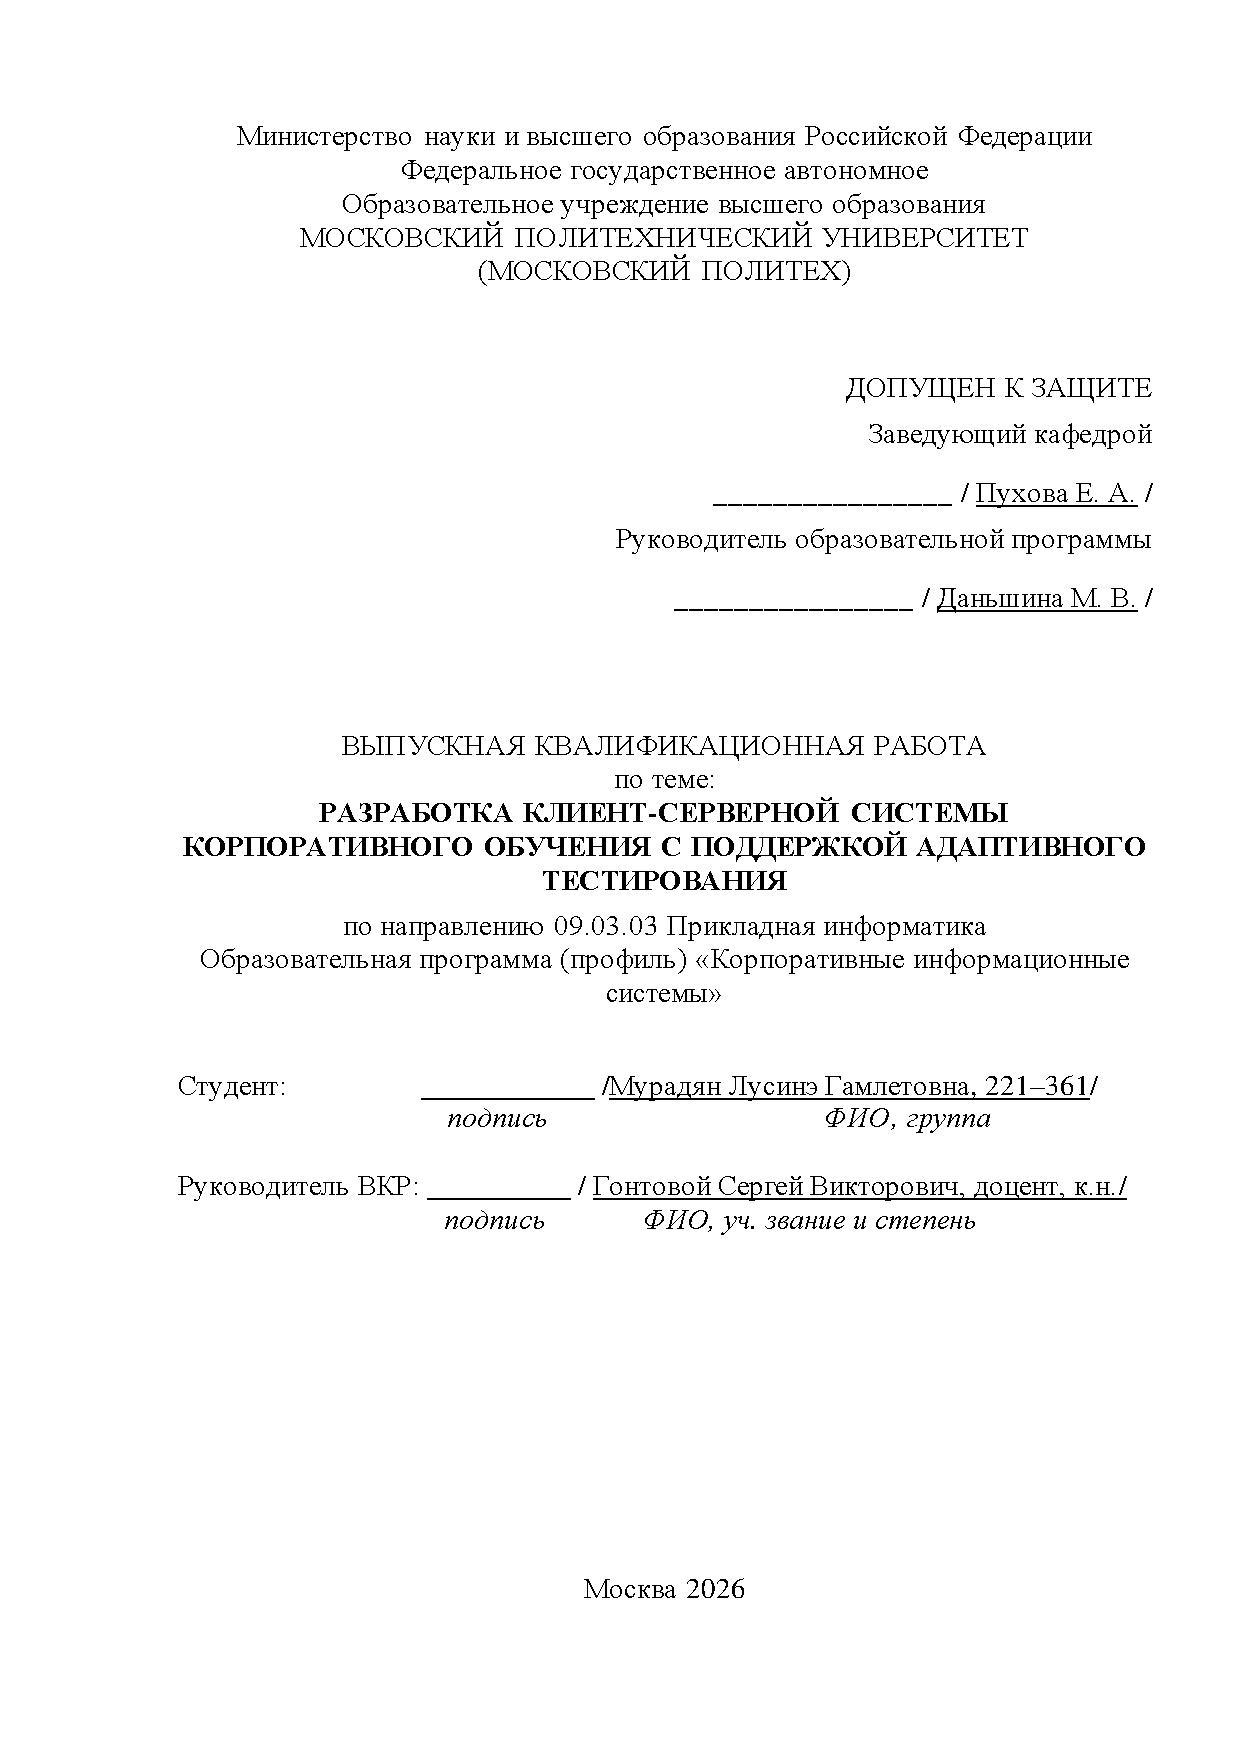
\includepdf[pages=1]{./extra/Title.pdf}
\newpage
\begin{center}
{\fontsize{14pt}{21pt}\selectfont\textbf{\MakeUppercase{Спецификация требований к системе}}\par}
\end{center}

\subsection*{1. Общее описание}

\subsubsection*{1.1. Цель создания}

Целью разработки является создание клиент-серверной системы корпоративного обучения с поддержкой адаптивного тестирования, предназначенной для персонализации учебного процесса сотрудников компаний и студентов вузов и для предоставления организациям удобных средств управления курсами и аналитики результатов обучения.

\subsubsection*{1.2. Границы проекта}

В проект входит реализация следующих компонентов системы:
\begin{itemize}
  \item серверное приложение с REST-API и базой данных для хранения информации об организациях, пользователях, курсах, уроках, тестах, результатах и профилях знаний;
  \item веб-панель администратора и преподавателя для управления курсами, пользователями, назначениями и аналитикой;
  \item мобильное приложение для обучающихся, обеспечивающее прохождение курсов и тестов, получение рекомендаций и просмотр личного прогресса.
\end{itemize}

Адаптивное тестирование реализуется на уровне подбора вопросов и рекомендаций по повторению тем.  
В состав проекта \textbf{не} входят: интеграции с платёжными сервисами, сложные механизмы авторизации через внешние корпоративные каталоги (AD/LDAP), полноценный редактор сложных мультимедийных курсов и продвинутые функции массового рассылочного сервиса.

\subsubsection*{1.3. Окружение системы}

Система разрабатывается как самостоятельное клиент-серверное веб-приложение с мобильным клиентом. Серверная часть разворачивается в облаке или на сервере организации и взаимодействует:
\begin{itemize}
  \item с веб-браузером администратора и преподавателя (веб-панель);
  \item с мобильным приложением обучающегося по HTTPS через REST-API;
  \item при необходимости — с внешними службами отправки e-mail и push-уведомлений.
\end{itemize}

Система может использоваться как автономное решение или как часть инфраструктуры организации, интегрируясь при необходимости с существующими учетными записями через отдельный адаптер (вне рамок текущего проекта).

\subsubsection*{1.4. Характеристики пользователей}

В системе предполагаются следующие основные роли пользователей:
\begin{itemize}
  \item \textbf{Обучающийся} — сотрудник или студент, проходящий назначенные курсы, выполняющий тесты и просматривающий свой прогресс.
  \item \textbf{Преподаватель / автор курса} — пользователь, создающий и редактирующий курсы, уроки и тесты, просматривающий результаты по своим курсам.
  \item \textbf{Администратор организации} — пользователь, управляющий списком пользователей и их ролями, назначающий курсы группам и отдельным пользователям, просматривающий агрегированную аналитику.
  \item \textbf{Системный администратор} — пользователь, отвечающий за создание и настройку организаций (тенантов), параметры системы и доступ к административным функциям сервера.
\end{itemize}

\subsubsection*{1.5. Предположения и зависимости}

Предположения:
\begin{itemize}
  \item пользователи имеют доступ к интернету и современным веб-браузерам / мобильным устройствам на Android или iOS;
  \item организации самостоятельно формируют и предоставляют учебный контент (курсы, тесты, материалы) в цифровом виде;
  \item количество одновременных пользователей и курсов соответствует типовой нагрузке учебных и корпоративных систем среднего масштаба.
\end{itemize}

Зависимости:
\begin{itemize}
  \item доступность внешних сервисов отправки e-mail и push-уведомлений, если они используются;
  \item доступность инфраструктуры размещения серверной части (облачный провайдер или сервер организации);
  \item своевременное предоставление данных о пользователях и организационной структуре со стороны заказчика.
\end{itemize}

\subsubsection*{1.6. Термины и соглашения}

\begin{itemize}
  \item \textbf{LMS} — система управления обучением (Learning Management System).
  \item \textbf{Тенант} — логически изолированная организация (компания, вуз) в рамках общей системы.
  \item \textbf{Курс} — логическая единица обучения, состоящая из модулей, уроков и тестов.
  \item \textbf{Адаптивное тестирование} — режим тестирования, при котором состав и сложность заданий, а также рекомендации зависят от результатов пользователя.
  \item \textbf{REST-API} — программный интерфейс для взаимодействия клиентских приложений с сервером по протоколу HTTP(S).
\end{itemize}

\subsection*{2. Детальные требования}

\subsubsection*{2.1. Требования к внешним интерфейсам}

\paragraph{2.1.1. Интерфейсы пользователя (UI)}

\begin{itemize}
  \item Веб-панель администратора и преподавателя должна предоставлять доступ к управлению курсами, пользователями, назначениями и аналитическими отчётами через современный веб-браузер.
  \item Мобильное приложение должно предоставлять обучающемуся простой и минималистичный интерфейс: список курсов, модулей, тестов, экран прохождения теста и экран рекомендаций.
  \item Навигация должна быть интуитивной: не более 3 кликов от главного экрана до начала урока или теста.
  \item В интерфейсе должны отображаться прогресс по курсу, статус модулей и результаты тестов.
\end{itemize}

Макеты экранов и схемы навигации приводятся в приложении к спецификации.

\paragraph{2.1.2. Аппаратные интерфейсы}

Специальные аппаратные интерфейсы не требуются. Достаточно стандартных возможностей персональных компьютеров и мобильных устройств (экран, клавиатура/сенсорный ввод, сеть).

\paragraph{2.1.3. Программные интерфейсы}

\begin{itemize}
  \item Система предоставляет REST-API для взаимодействия мобильного приложения и веб-панели с сервером.
  \item Формат обмена данными — JSON поверх HTTPS.
  \item В перспективе возможна интеграция с внешними системами (например, сервисами аутентификации или корпоративными порталами) через отдельные эндпоинты API.
\end{itemize}

\paragraph{2.1.4. Интерфейсы связи и коммуникации}

\begin{itemize}
  \item Весь сетевой обмен должен происходить по протоколу HTTPS.
  \item Поддерживается работа через интернет и внутренние корпоративные сети.
  \item Для уведомлений могут использоваться e-mail и push-уведомления мобильных платформ.
\end{itemize}

\subsubsection*{2.2. Функциональные требования}

Ниже приведён перечень ключевых функциональных требований (FR).

\paragraph{Модуль аутентификации и управления пользователями}

\textbf{FR-01. Регистрация пользователя}  
Система должна предоставлять возможность регистрации нового пользователя с указанием имени, e-mail и пароля либо импорта пользователя администратором из списка организации.

\textbf{FR-02. Аутентификация}  
Пользователь должен иметь возможность входа в систему по e-mail и паролю. При нескольких неудачных попытках входа возможна временная блокировка учётной записи.

\textbf{FR-03. Управление ролями пользователей}  
Администратор организации должен иметь возможность назначать пользователям роли «обучающийся», «преподаватель» или «администратор».

\paragraph{Модуль управления курсами}

\textbf{FR-04. Создание и редактирование курса}  
Преподаватель или администратор может создавать курсы, добавлять модули, уроки и тесты, редактировать их структуру и содержимое.

\textbf{FR-05. Назначение курсов пользователям и группам}  
Администратор организации может назначать курсы отдельным пользователям или группам, устанавливать дедлайны и обязательность прохождения.

\textbf{FR-06. Просмотр и прохождение курсов обучающимся}  
Обучающийся должен видеть список назначенных курсов, состояние прохождения и иметь возможность открывать уроки и тесты.

\paragraph{Модуль тестирования и адаптивности}

\textbf{FR-07. Прохождение тестов}  
Система должна предоставлять обучающемуся вопросы теста, принимать ответы и фиксировать результаты (баллы, время, попытки).

\textbf{FR-08. Адаптивный выбор заданий}  
Система должна подстраивать состав и сложность вопросов на основе предыдущих ответов и уровня освоения тем: чаще предлагать задания по слабым темам и реже по уже освоенным.

\textbf{FR-09. Формирование рекомендаций}  
После прохождения теста система формирует рекомендации: список тем для повторения, дополнительные уроки и тесты, предлагаемые к прохождению.

\paragraph{Модуль аналитики и отчётности}

\textbf{FR-10. Просмотр личного прогресса обучающегося}  
Обучающийся должен видеть завершённые курсы, результаты тестов, динамику освоения тем.

\textbf{FR-11. Отчёты администратора и преподавателя}  
Администратор и преподаватель должны иметь возможность просматривать отчёты по курсам, группам и отдельным пользователям: процент прохождения, проблемные темы, количество попыток.

\subsubsection*{2.3. Нефункциональные требования}

\paragraph{Производительность}

\textbf{NFR-01.} Время ответа сервера на типовые запросы (получение списка курсов, отправка результатов теста) не должно превышать 2 секунд при средней нагрузке.  

\textbf{NFR-02.} Система должна поддерживать одновременную работу не менее 100 активных пользователей без заметного ухудшения отклика.

\paragraph{Безопасность}

\textbf{NFR-03.} Весь сетевой трафик между клиентами и сервером должен шифроваться (HTTPS).  

\textbf{NFR-04.} Пароли пользователей хранятся только в виде криптографических хэшей.  

\textbf{NFR-05.} Должно вестись журналирование ключевых событий безопасности (вход, смена пароля, изменение прав доступа).

\paragraph{Удобство использования}

\textbf{NFR-06.} Новый пользователь должен освоить основные функции мобильного приложения (поиск курса, запуск урока и теста) за время не более 30 минут.  

\textbf{NFR-07.} Интерфейс должен быть адаптирован для работы на типичных экранах смартфонов и не требовать горизонтальной прокрутки.

\paragraph{Надёжность и отказоустойчивость}

\textbf{NFR-08.} Система должна быть доступна не менее 99\% времени в течение учебного периода (при условии корректной настройки инфраструктуры).  

\textbf{NFR-09.} Время восстановления после отказа (перезапуск сервера, восстановление из резервной копии) не должно превышать 30 минут.

\paragraph{Масштабируемость}

\textbf{NFR-10.} Архитектура системы должна позволять масштабировать серверную часть по горизонтали (несколько экземпляров приложения и БД) при росте числа организаций и пользователей.

\paragraph{Локализация}

\textbf{NFR-11.} Система должна поддерживать как минимум русский и английский язык интерфейса; структура данных должна позволять добавление дополнительных языков.

\end{document}
